\documentclass[conference]{IEEEtran}
\IEEEoverridecommandlockouts

\usepackage{cite}
\usepackage{amsmath,amssymb,amsfonts}
\usepackage{algorithm}
\usepackage{algpseudocode}
\usepackage{graphicx}
\usepackage{textcomp}
\usepackage{xcolor}
\usepackage{booktabs}
\usepackage{tabularx}
\usepackage{multirow}
\usepackage{tikz}
\usetikzlibrary{arrows.meta,positioning,shapes.geometric,fit,backgrounds}
\usepackage[hidelinks]{hyperref}

\begin{document}

\title{DietSense: A Conversational Domain AI Agent for Dietary Logging and Nutrition Analysis in Taiwan}

\author{
\IEEEauthorblockN{Jin-Song Wu}
\IEEEauthorblockA{AIoT Research Project\\
Taipei, Taiwan\\
wujin910504@gmail.com}
}

\maketitle

\begin{abstract}
Dietary self-monitoring has been used in behavioral weight-management interventions, yet adherence metrics and outcomes vary across studies. In Taiwan, everyday meals frequently involve mixed dishes, local terminology, and ambiguous portion descriptions that challenge conventional database-search workflows. This paper presents DietSense, a research proposal for a Traditional Chinese conversational domain AI agent designed for traceable dietary logging and nutrition analysis in Taiwan. Rather than allowing a large language model (LLM) to generate nutrient values from parametric memory, DietSense separates language understanding and tool orchestration from verified data retrieval and deterministic calculation. The proposed architecture comprises eight conceptual modules governed by an explicit trust boundary: user inputs and retrieved text are treated as untrusted data, candidate records are retrieved from USDA FoodData Central and versioned Taiwan food-composition and local-recipe sources, and an Analytics Engine computes energy and macronutrients deterministically while preserving null/unknown values without zero-imputation. When food identity, preparation, or portion mass is insufficiently specified, the agent performs bounded multi-turn clarification or degrades gracefully to partial estimates, evidence-bounded plausible ranges, or text-only logs. Domain safety guardrails restrict responses to general informational support and exclude clinical diagnosis or prescription. We further specify a prospective evaluation protocol comprising 500 annotated Traditional Chinese meal descriptions compared against a fixed manual-search baseline and a 20-participant, 7-day feasibility study. No experimental results, system implementation, or clinical validation are reported at this proposal stage.
\end{abstract}

\begin{IEEEkeywords}
Conversational AI agent, dietary self-monitoring, nutrition informatics, retrieval-augmented generation, portion estimation, uncertainty communication, Taiwanese cuisine.
\end{IEEEkeywords}

\section{Introduction}
Global and local public-health statistics underscore the importance of dietary monitoring as a research domain. The World Health Organization (WHO) estimates that approximately 2.6 billion adults worldwide were overweight in 2024, including 940 million adults living with obesity~\cite{who2026obesity}. In Taiwan, the Health Promotion Administration (HPA) reported that 51.3\% of adults aged 18 years or older met the combined overweight-or-obesity criterion in the 2020--2024 National Nutrition and Health Survey~\cite{hpa2026obesity}. While these prevalence figures motivate accessible dietary tracking tools, they do not establish that any single logging interface prevents or treats disease. A systematic review of 59 behavioral weight-loss interventions found that dietary self-monitoring may support weight management, but heterogeneous adherence definitions limit conclusions regarding usage intensity and outcomes~\cite{raber2021systematic}.

Conventional database-driven food logging requires users to search food items, reconcile preparation states, and estimate portion weights. Systematic reviews demonstrate that portion-size estimation aids vary substantially in validation quality~\cite{amoutzopoulos2020portion}, and image-based dietary assessment methods exhibit significant inter-study heterogeneity~\cite{ho2020validity}. Although authoritative food composition resources exist---including USDA FoodData Central (FDC)~\cite{usda_fdc} and the Taiwan Food and Drug Administration (TFDA) Food Nutrition Composition Database~\cite{tfda_database}---everyday Taiwanese meals such as ``one bowl of beef noodle soup with egg, half the broth consumed'' omit bowl volume, noodle mass, meat cut, recipe oil, and broth intake. Producing a single precise calorie figure from a superficially matched database entry masks portion and recipe assumptions.

Recent advances in large language models (LLMs) and retrieval-augmented generation (RAG)~\cite{lewis2020rag} enable flexible natural-language parsing and tool coordination~\cite{yao2023react}, while recent nutrition informatics studies have explored free-text food mapping~\cite{lemay2026foodmapper}, retrieval-augmented food classification~\cite{zhou2026nutrirag}, domain-aligned food LLMs~\cite{gjorgjevikj2026foodyllm}, text-based nutrient estimation~\cite{lawabni2026text,cao2026chinese}, and image-based dietary assessment in Taiwan~\cite{chen2025diabot}. Consequently, we do not claim that LLM-based dietary tracking or Chinese food estimation is unexplored. Instead, we define a focused, testable research gap: whether an end-to-end Traditional Chinese conversational workflow combining structured retrieval, bounded clarification, deterministic calculation, and field-level provenance can produce traceable nutrition estimates for Taiwanese mixed dishes while quantifying error and interaction burden against a fixed manual-search baseline.

This paper makes four prospective contributions:
\begin{enumerate}
    \item A formal, trust-bounded eight-module conversational agent architecture tailored to Traditional Chinese dietary logging.
    \item A deterministic nutrition calculation and evidence-bounded plausible-range methodology that separates unknown values from zero and prohibits uncalibrated confidence intervals.
    \item A non-blocking multi-intent agent algorithm with bounded clarification, graceful degradation, and versioned safety checks.
    \item A reproducible prospective evaluation design featuring a 500-item stratified Taiwanese meal dataset, a 4-tier reference labeling protocol, and a 20-adult, 7-day feasibility study.
\end{enumerate}

\section{Related Work}
\subsection{Food Language Understanding and Entity Linking}
Food natural language processing (NLP) distinguishes entity extraction from database normalization. Popovski et al.~\cite{popovski2019foodbase} introduced the FoodBase corpus of curated recipe annotations, and Stojanov et al.~\cite{stojanov2021foodner} fine-tuned BERT and BioBERT models for food named-entity recognition (NER), achieving macro-F1 scores of 73.39\%--78.96\% across ontology subsets. Feher et al.~\cite{feher2023fewshot} compared string matching, classical machine learning, and few-shot Siamese models for food entity linking. More recently, Ogrinc et al.~\cite{ogrinc2024zeroshot} evaluated ChatGPT-3.5 and GPT-4 in zero-shot food NER and ontology linking. However, these benchmarks focus primarily on English recipes and scientific abstracts rather than colloquial Traditional Chinese meal logs, and entity linking alone does not resolve portion mass or nutrient provenance.

\subsection{RAG, Tool-Using Agents, and LLM Nutrition Estimation}
Lewis et al.~\cite{lewis2020rag} formalized RAG for knowledge-intensive NLP, and Yao et al.~\cite{yao2023react} introduced ReAct to interleave reasoning traces with external tool actions. In nutrition informatics, Thames et al.~\cite{thames2021nutrition5k} released Nutrition5k for visual nutrient prediction from U.S. cafeteria meals, and Yan et al.~\cite{yan2025dietai24} proposed DietAI24, integrating multimodal LLMs, RAG, and FNDDS for image-based nutrient estimation. DietAI24 demonstrates that combining LLMs, RAG, and food databases is already established for image workflows.

Recent 2026 studies further address text-based dietary analysis. Lemay et al.~\cite{lemay2026foodmapper} evaluated hybrid semantic retrieval and LLM mapping (FoodMapper) on ASA24/FooDB and NHANES/DFG2 benchmarks (90.7\% and 65.4\% accuracy, respectively). Zhou et al.~\cite{zhou2026nutrirag} proposed NutriRAG for retrieval-augmented classification of free-text food logs (micro-F1 82.24\%). Gjorgjevikj et al.~\cite{gjorgjevikj2026foodyllm} trained FoodyLLM on domain-aligned nutrition QA tasks. Lawabni et al.~\cite{lawabni2026text} and Cao et al.~\cite{cao2026chinese} evaluated text-based LLM nutrient estimation against the U.S. NCC database and the Chinese Food Composition Table, respectively, finding stronger agreement for energy and macronutrients than for micronutrients or composite dishes. In Taiwan, Chen et al.~\cite{chen2025diabot} validated Diabot-GPT-4o for image-based dietary assessment among 57 dietetic trainees against weighed food records.

\subsection{Nutrition Domain Knowledge and Safety Boundaries}
Deterministic nutrient scaling relies on matching food identity, raw/cooked state, edible portion, and source nutrient definitions. Predictive energy equations such as Mifflin--St Jeor~\cite{mifflin1990ree} estimate resting energy expenditure (REE) rather than directly measuring basal metabolic rate, and the National Academies Energy DRI report emphasizes systematic measurement error in self-reported intake~\cite{nasem2023dri}. Dynamic energy-balance modeling~\cite{hall2011bodyweight} shows that bodyweight change cannot be reduced to a fixed linear single-day calorie rule. Moreover, personalized nutrition findings such as glycemic-response prediction~\cite{zeevi2015personalized} or the DIETFITS trial~\cite{gardner2018dietfits} do not support automated calorie prescriptions. Finally, systematic reviews examine associations between weight-related self-monitoring apps and disordered eating symptoms~\cite{roth2024selfmonitoring,anderberg2025apps}, reinforcing the need for non-diagnostic, non-punitive safety boundaries informed by clinical care frameworks such as NICE NG69~\cite{nice2020ng69}. Table~\ref{tab:related_work} summarizes how DietSense relates to representative prior work.

\begin{table*}[t]
\centering
\caption{Comparison of Representative Prior Work and the Proposed DietSense Framework}
\label{tab:related_work}
\renewcommand{\arraystretch}{1.15}
\begin{tabularx}{\textwidth}{@{}l l l l X@{}}
\toprule
\textbf{Study / System} & \textbf{Modality / Lang.} & \textbf{Core Method} & \textbf{Primary Data Source} & \textbf{Key Limitation Relative to DietSense} \\
\midrule
FoodNER~\cite{stojanov2021foodner} & Text (EN) & Fine-tuned BERT/BioBERT & FoodBase / FoodOn & NER only; no portion or nutrient calculation. \\
DietAI24~\cite{yan2025dietai24} & Image (EN) & MLLM + RAG & U.S. FNDDS & Image-centric U.S. workflow; no TW text dialogue. \\
FoodMapper~\cite{lemay2026foodmapper} & Text (EN) & Hybrid semantic + LLM & FooDB / DFG2 & Static mapping; no interactive clarification loop. \\
NutriRAG~\cite{zhou2026nutrirag} & Text (EN) & RAG + GPT-4 classification & Trial food logs & Food-group classification; not nutrient provenance. \\
FoodyLLM~\cite{gjorgjevikj2026foodyllm} & Text (EN) & Domain-aligned LLM & Curated QA tasks & Benchmark QA; no deterministic audit pipeline. \\
Lawabni et al.~\cite{lawabni2026text} & Text (EN) & Direct LLM querying & U.S. NCC & High variance on mixed dishes/micronutrients. \\
Cao et al.~\cite{cao2026chinese} & Text (ZH-CN) & Direct LLM querying & China FCT & Standard single items; no TW mixed-dish dialogue. \\
Diabot-GPT-4o~\cite{chen2025diabot} & Image (TW) & Multimodal GPT-4o & Weighed TW records & Image-based trainee study; not text-first agent. \\
\textbf{DietSense (Proposed)} & \textbf{Text (ZH-TW)} & \textbf{LLM + RAG + Det. Calc.} & \textbf{USDA FDC + TW sources} & \textbf{Prospective proposal; unimplemented/untested.} \\
\bottomrule
\end{tabularx}
\end{table*}

\section{Proposed Methodology}
\subsection{Design Principles and Trust Separation}
DietSense enforces strict separation between language interpretation and numerical computation:
\begin{itemize}
    \item \textbf{Deterministic Numeric Authority:} LLMs parse user intent, food mentions, preparation cues, and portion spans, and generate clarification prompts, but never fabricate nutrient values or override calculation formulas.
    \item \textbf{Null vs.\ Zero Distinction:} Missing nutrient fields are explicitly represented as \texttt{null}/\texttt{unknown} with reason codes; missing values are never imputed as $0$.
    \item \textbf{Field-Level Provenance:} Every numeric output carries source ID, version/snapshot date, food ID, food state, unit, and formula version.
\end{itemize}

\subsection{Deterministic Nutrient Calculation}
For a verified food candidate $c$ with confirmed portion mass $m_c > 0$ (in grams) and source nutrient density $d_{c,k} \ge 0$ (in kcal/100\,g for energy or g/100\,g for macronutrient $k$), the deterministic nutrient amount $N_{c,k}$ is computed as:
\begin{equation}
N_{c,k} = m_c \cdot \frac{d_{c,k}}{100}.
\label{eq:scaling}
\end{equation}
For a multi-ingredient meal $M$ consisting of verified components $i \in \{1, \dots, n\}$ with effective consumed mass $m_i = m_i^{\text{served}} (1 - \ell_i)$, where $\ell_i \in [0, 1)$ denotes an explicit leftover fraction, the meal total for nutrient $k$ is:
\begin{equation}
N_{M,k} =
\begin{cases}
\sum_{i=1}^{n} m_i \cdot \dfrac{d_{i,k}}{100}, & \text{if } d_{i,k} \neq \texttt{null}\ \forall i, \\[8pt]
\texttt{partial}\!\left(\sum_{i \in \mathcal{V}_k} N_{i,k}\right), & \text{otherwise},
\end{cases}
\label{eq:aggregation}
\end{equation}
where $\mathcal{V}_k = \{i : d_{i,k} \neq \texttt{null}\}$. Incomplete totals explicitly report coverage counts rather than silently treating missing components as zero.

\subsection{Evidence-Bounded Plausible Estimate Ranges}
When portion mass or candidate identity has explicit, source-backed lower and upper bounds $[m^{\text{low}}, m^{\text{high}}]$ and $[d_k^{\text{low}}, d_k^{\text{high}}]$ with $0 < m^{\text{low}} \le m^{\text{high}}$ and $0 \le d_k^{\text{low}} \le d_k^{\text{high}}$, DietSense constructs an evidence-bounded plausible range:
\begin{equation}
R_k = \left[\frac{m^{\text{low}} d_k^{\text{low}}}{100},\; \frac{m^{\text{high}} d_k^{\text{high}}}{100}\right].
\label{eq:range}
\end{equation}
Crucially, $R_k$ is an assumption-conditional interval and is \emph{never} labeled a statistical confidence interval absent external calibration. Retrieval ranking scores are used solely for candidate ordering and are never converted into arbitrary percentage error bands.

\subsection{Optional Energy Reference Estimation}
Only when an eligible adult user ($\ge 18$ years, non-pregnant/lactating, no self-reported clinical diet therapy) explicitly requests an energy reference with complete anthropometric inputs, DietSense computes an optional REE estimate via the Mifflin--St Jeor equation~\cite{mifflin1990ree}:
\begin{equation}
\text{REE}_{\text{est}} = 10 w + 6.25 h - 5 a + s, \quad s \in \{+5, -161\},
\label{eq:mifflin}
\end{equation}
where $w$ is weight (kg), $h$ is height (cm), $a$ is age (years), and $s$ denotes the published male/female constant. If a user-selected activity factor $\alpha$ is provided, $\text{TDEE}_{\text{est}} = \text{REE}_{\text{est}} \cdot \alpha$ is reported as a secondary population estimate, never as a clinical prescription.

\subsection{Non-Blocking Multi-Intent Agent Algorithm}
Following the detailed system specification, DietSense models clarification as an asynchronous cross-request state transition rather than a blocking server loop. Algorithm~\ref{alg:agent} formalizes request handling across all supported intents (\texttt{log\_food}, \texttt{query\_nutrition}, \texttt{analyze}, \texttt{recommend}) with bounded clarification turns ($t \le T_{\max}$, default $T_{\max}=2$) and pre-/post-execution safety gates.

\begin{algorithm}[t]
\caption{Non-Blocking Multi-Intent Request Handling}
\label{alg:agent}
\begin{algorithmic}[1]
\Require User input $u$, session state $S$ (policy version $v_p$, max turns $T_{\max}$)
\Ensure Validated response envelope $E$, updated state $S'$
\State $\sigma_{\text{pre}} \gets \text{SafetyPreCheck}(u, v_p)$
\If{$\sigma_{\text{pre}}.\text{status} \in \{\texttt{refuse}, \texttt{restrict}, \texttt{refer}\}$}
    \State \Return $\text{RenderSafetyTemplate}(\sigma_{\text{pre}}), S$
\EndIf
\State $P \gets \text{ParseAndValidateSchema}(u)$
\If{$P.\text{status} \neq \texttt{success}$}
    \State \Return $\text{SafeParseFallback}(P), S$
\EndIf
\If{$P.\text{intent} = \texttt{log\_food}$}
    \State $C \gets \text{RetrieveVerifiedCandidates}(P.\text{entities})$
    \If{$\text{NeedsClarification}(P, C)$ \textbf{and} $S.t < T_{\max}$}
        \State $q \gets \text{SelectHighestImpactQuestion}(P, C)$
        \State $S' \gets \text{PersistMinimalState}(S, P, C, t{+}1)$
        \State \Return $\text{RenderClarification}(q, \texttt{allow\_skip}), S'$
    \EndIf
    \State $R \gets \text{DeterministicAnalytics}(P, C)$ \Comment{Eqs.~(\ref{eq:scaling})--(\ref{eq:range})}
\ElsIf{$P.\text{intent} = \texttt{query\_nutrition}$}
    \State $R \gets \text{AnswerFromVerifiedCandidates}(P.\text{query})$
\ElsIf{$P.\text{intent} = \texttt{analyze}$}
    \State $R \gets \text{AggregateDailyLog}(S.\text{log}, P.\text{date}, S.\text{tz})$
\ElsIf{$P.\text{intent} = \texttt{recommend}$}
    \State $R \gets \text{GeneralInfoIfAllowed}(S.\text{log}, \sigma_{\text{pre}}, v_p)$
\Else
    \State \Return $\text{UnsupportedIntentResponse}(), S$
\EndIf
\State $\sigma_{\text{post}} \gets \text{SafetyPostCheck}(R, \sigma_{\text{pre}}, v_p)$
\State $E \gets \text{RenderValidatedEnvelope}(R, \sigma_{\text{post}})$
\State \Return $E$ (with confirmation gate if draft log), $S'$
\end{algorithmic}
\end{algorithm}

\section{System Architecture}
\subsection{Eight-Module Conceptual Architecture}
To maintain consistency with the detailed system design specification, DietSense is structured into eight conceptual modules (Fig.~\ref{fig:architecture}), distinct from backing storage infrastructure:
\begin{enumerate}
    \item \textbf{User / Application Layer (M1):} Captures Traditional Chinese meal input, displays structured previews with provenance and assumptions, and enforces explicit user confirmation, edit, skip, and deletion controls.
    \item \textbf{Input Processing (M2):} Preserves raw text, normalizes whitespace/width, extracts intent and food/portion/preparation spans, and validates outputs against versioned schemas.
    \item \textbf{Planner / Reasoning (M3):} Executes a finite-state workflow orchestrating retrieval, bounded clarification, analytics, and terminal fallback states.
    \item \textbf{Data Retrieval (M4):} Queries licensed, versioned nutrition sources (USDA FDC, candidate TFDA database, curated local-recipe index) and returns ranked \texttt{NutritionCandidate} objects with field-level provenance.
    \item \textbf{Analytics Engine (M5):} Executes pure deterministic functions for unit validation, nutrient scaling, ingredient aggregation, daily summaries, and optional REE/TDEE estimation.
    \item \textbf{Domain Knowledge (M6):} Stores versioned unit conversions, source priority rules, population dietary guidance scope, and safety policy definitions.
    \item \textbf{Decision / Recommendation (M7):} Combines calculation completeness and safety decisions (\texttt{allow\_general}, \texttt{restrict}, \texttt{refuse}, \texttt{refer}) to determine permissible response plans.
    \item \textbf{Output / Interaction (M8):} Renders structured \texttt{ResponseEnvelope} payloads exposing units, sources, assumptions, unknown fields, and plausible ranges without performing post-hoc arithmetic.
\end{enumerate}

\begin{figure*}[t]
\centering
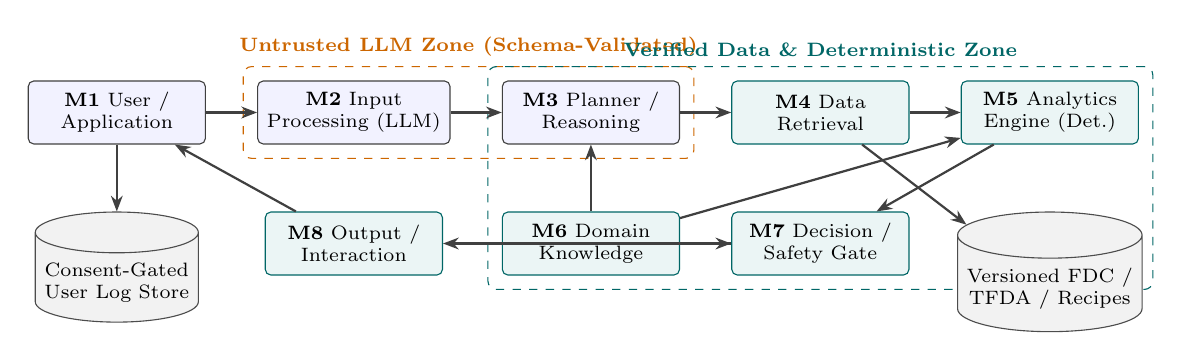
\begin{tikzpicture}[
    node distance=0.55cm and 0.65cm,
    box/.style={rectangle, draw=black!75, rounded corners=2pt, minimum width=2.25cm, minimum height=0.8cm, align=center, font=\scriptsize, fill=blue!5},
    trust/.style={rectangle, draw=teal!80!black, rounded corners=2pt, minimum width=2.25cm, minimum height=0.8cm, align=center, font=\scriptsize, fill=teal!8},
    store/.style={cylinder, shape border rotate=90, draw=black!70, aspect=0.25, minimum width=1.9cm, minimum height=0.75cm, align=center, font=\scriptsize, fill=gray!10},
    arr/.style={-{Stealth[length=2mm]}, thick, draw=black!75}
]
\node[box] (m1) {\textbf{M1} User /\\Application};
\node[box, right=of m1] (m2) {\textbf{M2} Input\\Processing (LLM)};
\node[box, right=of m2] (m3) {\textbf{M3} Planner /\\Reasoning};
\node[trust, right=of m3] (m4) {\textbf{M4} Data\\Retrieval};
\node[trust, right=of m4] (m5) {\textbf{M5} Analytics\\Engine (Det.)};

\node[trust, below=0.85cm of m3] (m6) {\textbf{M6} Domain\\Knowledge};
\node[trust, below=0.85cm of m4] (m7) {\textbf{M7} Decision /\\Safety Gate};
\node[trust, below=0.85cm of m2] (m8) {\textbf{M8} Output /\\Interaction};

\node[store, below=0.85cm of m1] (logdb) {Consent-Gated\\User Log Store};
\node[store, below=0.85cm of m5] (nutdb) {Versioned FDC /\\TFDA / Recipes};

\draw[arr] (m1) -- (m2);
\draw[arr] (m2) -- (m3);
\draw[arr] (m3) -- (m4);
\draw[arr] (m4) -- (m5);
\draw[arr] (m6) -- (m3);
\draw[arr] (m6) -- (m5);
\draw[arr] (m6) -- (m7);
\draw[arr] (m5) -- (m7);
\draw[arr] (m7) -- (m8);
\draw[arr] (m8) -- (m1);
\draw[arr] (m1) -- (logdb);
\draw[arr] (m4) -- (nutdb);

\begin{scope}[on background layer]
    \node[draw=orange!80!black, dashed, rounded corners=3pt, fit=(m2)(m3), inner sep=5pt, label={[font=\scriptsize\bfseries, text=orange!80!black]above:Untrusted LLM Zone (Schema-Validated)}] {};
    \node[draw=teal!80!black, dashed, rounded corners=3pt, fit=(m4)(m5)(m6)(m7), inner sep=5pt, label={[font=\scriptsize\bfseries, text=teal!80!black]above:Verified Data \& Deterministic Zone}] {};
\end{scope}
\end{tikzpicture}
\caption{Eight-module conceptual architecture of DietSense illustrating the trust boundary separating LLM-based language parsing and orchestration from schema-validated retrieval, deterministic analytics, and versioned safety gates.}
\label{fig:architecture}
\end{figure*}

\subsection{Data Contracts and Graceful Degradation}
Inter-module communication uses versioned data contracts: \texttt{UserInput}, \texttt{FoodEntity}, \texttt{PortionEstimate}, \texttt{NutritionCandidate}, \texttt{NutritionRecord}, \texttt{CalculationResult}, \texttt{ClarificationRequest}, \texttt{DailySummary}, and \texttt{SafetyDecision}. All timestamps follow ISO~8601 with explicit timezone; mass uses grams (g) and energy uses kilocalories (kcal). Retrieved documents and user text are treated as untrusted inputs to mitigate prompt injection. Under API timeouts, zero candidates, unit mismatches, or exhausted clarification turns, DietSense transitions to explicit terminal states (\texttt{confirmed}, \texttt{draft}, \texttt{text\_only}, or \texttt{incomplete}) without fabricating numeric estimates. Table~\ref{tab:contracts} summarizes core data contracts and failure policies.

\begin{table}[t]
\centering
\caption{Core Data Contracts and Degradation Rules}
\label{tab:contracts}
\renewcommand{\arraystretch}{1.12}
\begin{tabularx}{\columnwidth}{@{}l X@{}}
\toprule
\textbf{Contract} & \textbf{Key Fields \& Integrity Rule} \\
\midrule
\texttt{FoodEntity} & Original span, normalized name, \texttt{food\_type}, explicit ingredients; never infer recipe from dish name. \\
\texttt{PortionEstimate} & Quantity, unit, \texttt{mass\_g}, optional \texttt{[low, high]}, \texttt{leftover\_fraction}, assumptions; no default bowl mass. \\
\texttt{NutritionCandidate} & \texttt{source\_id}, \texttt{source\_version}, \texttt{food\_id}, \texttt{nutrients\_per\_100g}, \texttt{value\_basis}; score is rank-only. \\
\texttt{CalculationResult} & \texttt{formula\_version}, \texttt{inputs\_hash}, nullable nutrients, \texttt{completeness}; missing fields remain \texttt{null}. \\
\texttt{SafetyDecision} & \texttt{allow\_general}/\texttt{restrict}/\texttt{refuse}/\texttt{refer}, \texttt{policy\_version}, \texttt{review\_status=pending}. \\
\bottomrule
\end{tabularx}
\end{table}

\section{Experimental Design}
All datasets, baselines, metrics, and user studies described below are prospective research plans; no data collection or experimentation has been executed.

\subsection{Research Questions}
\begin{itemize}
    \item \textbf{RQ1 (Estimation Accuracy):} On a fixed Traditional Chinese Taiwanese meal benchmark, how accurately does DietSense identify foods and estimate energy and available macronutrients relative to reference labels?
    \item \textbf{RQ2 (Clarification, Provenance, and Fallbacks):} When key fields are missing or matches are weak, does DietSense elicit bounded clarifications, preserve field-level provenance, and avoid unsupported numeric outputs?
    \item \textbf{RQ3 (Workflow Feasibility):} Compared against a fixed, version-recorded manual-search logging baseline, how does DietSense perform in logging time, task completion, clarification burden, and subjective usability?
\end{itemize}

\subsection{Dataset Construction and Four-Tier Reference Labeling}
We plan to construct a stratified dataset of 500 Traditional Chinese meal descriptions spanning six categories: (1) packaged/single foods, (2) Taiwanese bento and staple combinations, (3) noodle soups with broth/topping ambiguity, (4) night-market and street mixed dishes (e.g., oyster omelet, fried chicken cutlet, bubble tea), (5) home-cooked/local recipes, and (6) deliberately ambiguous, contradictory, or safety-boundary cases. Natural and synthetic descriptions will be tagged separately.

Because reference nutrition values are not error-free ground truth, each item will be assigned a four-tier reference level: \textbf{Tier~A} (verified packaged label or official database match), \textbf{Tier~B} (standardized recipe with weighed ingredients and documented raw/cooked conversions), \textbf{Tier~C} (field-collected vendor meals with pre-/post-meal weighing and explicit oil/sauce uncertainty), and \textbf{Tier~D} (insufficient reference; evaluated solely for safe fallback/abstention and excluded from primary numeric error analysis). Two trained annotators will independently annotate entries using a frozen codebook, with a qualified dietitian adjudicating disagreements. Inter-annotator agreement will be reported using Cohen's $\kappa$ for categorical labels and intraclass correlation coefficients (ICC) with Bland--Altman analysis for continuous values. Group-aware splits by dish, recipe, vendor, and brand will prevent data leakage.

\subsection{Baselines, Metrics, and Feasibility Study}
The primary baseline is a version-locked manual-search-and-entry workflow using the same meal tasks and reference sources. An analytical baseline (direct database lookup with manual formula application) and optional ablations (no clarification vs.\ bounded clarification vs.\ LLM-only error analysis) are planned. Table~\ref{tab:metrics} defines the evaluation metrics.

\begin{table}[t]
\centering
\caption{Planned Evaluation Metrics and Reporting Rules}
\label{tab:metrics}
\renewcommand{\arraystretch}{1.12}
\begin{tabularx}{\columnwidth}{@{}l X@{}}
\toprule
\textbf{Dimension} & \textbf{Metric Definition \& Reporting} \\
\midrule
Food ID & Exact normalized Top-1 accuracy; dish accuracy; ingredient P/R/F1; candidate coverage rate. \\
Calorie Error & $\text{AE} = |\hat{y} - y|$ (kcal): MAE, median, IQR; $\text{APE}$ for $y>0$; proportion within $\pm 10\%$ and $\pm 20\%$. \\
Range Quality & Empirical coverage ($y \in [R^{\text{low}}, R^{\text{high}}]$) and mean width; never reported as statistical CI. \\
Macros & Protein, carbohydrate, fat, fiber MAE (g) over available fields with separate completeness rate. \\
Interaction & Logging time (median/IQR seconds), task completion rate, clarification turns, skip/abandon rate. \\
Provenance & Valid \texttt{source\_id/version/field} lineage rate; zero-provenance numeric output as safety-critical error. \\
Usability & System Usability Scale (SUS, 0--100)~\cite{brooke1996sus}, reported as distribution, not clinical efficacy. \\
\bottomrule
\end{tabularx}
\end{table}

We also plan a 20-adult, 7-day feasibility study comparing DietSense with the manual baseline using counterbalanced task assignment where feasible. Candidate thresholds from the original proposal ($>85\%$ within $\pm 20\%$, 60\% shorter logging time, SUS $>70$) are explicitly treated as unvalidated exploratory targets pending pilot calibration and protocol preregistration. Recruitment will not begin until institutional ethics/IRB approval, informed consent, privacy controls, and third-party LLM data-retention policies are finalized.

\section{Discussion and Limitations}
Several methodological and engineering limitations bound this proposal. First, our literature review was a targeted scoping search rather than a systematic review, and did not directly search native IEEE Xplore or ACM Digital Library interfaces; therefore, novelty is framed as a testable workflow question rather than a universal priority claim. Second, DietSense is currently unimplemented, and neither the 500-item dataset nor the 20-participant feasibility study has been executed. Third, text-only meal descriptions cannot directly observe hidden cooking oil, sauces, or unmeasured leftovers; consequently, some Taiwanese mixed dishes will legitimately degrade to \texttt{text\_only} or bounded ranges.

Fourth, from a safety and governance perspective, DietSense is not a medical device and does not replace registered dietitians. While removing the original proposal's universal 1,200\,kcal/day cutoff avoids an unvalidated clinical rule, all replacement safety policies, referral templates, and privacy/deletion workflows remain \texttt{pending\_professional\_review}. Fifth, a 20-participant, 7-day study is designed solely for operational feasibility and cannot support population generalization, subgroup inference, or weight-loss efficacy claims.

Finally, during specification consolidation, two material inconsistencies in earlier project documents were resolved using the detailed system design specification: (1) the eight conceptual modules follow the logical architecture (M1--M8 in Fig.~\ref{fig:architecture}) rather than treating database and API gateway infrastructure as conceptual modules 7 and 8; and (2) clarification is formalized as a non-blocking cross-request state machine (Algorithm~\ref{alg:agent}) rather than a blocking \texttt{while} loop.

\section{Conclusion}
This paper presented the research proposal, trust-bounded eight-module architecture, deterministic calculation methodology, and prospective evaluation design for DietSense, a Traditional Chinese conversational domain AI agent for dietary logging and nutrition analysis in Taiwan. By decoupling LLM-based language understanding from versioned nutrition retrieval, deterministic arithmetic, bounded clarification, and non-diagnostic safety guardrails, DietSense aims to make uncertainty and data provenance explicit in mixed-dish meal logging. Immediate next steps include auditing Taiwan food-composition source licensing and coverage, completing professional review of safety policies, preregistering the 500-item annotation protocol, and conducting pilot validation prior to prototype implementation and IRB-approved feasibility testing.

\bibliographystyle{IEEEtran}
\bibliography{references}

\end{document}
